\section{Proposed Architecture}
A better zoomable representation of these diagrams can be found in the github repository of this project in /doc/pflichtenheft/pics, where also the xml sources are.
\subsection{Overview}

\hspace{-3cm} 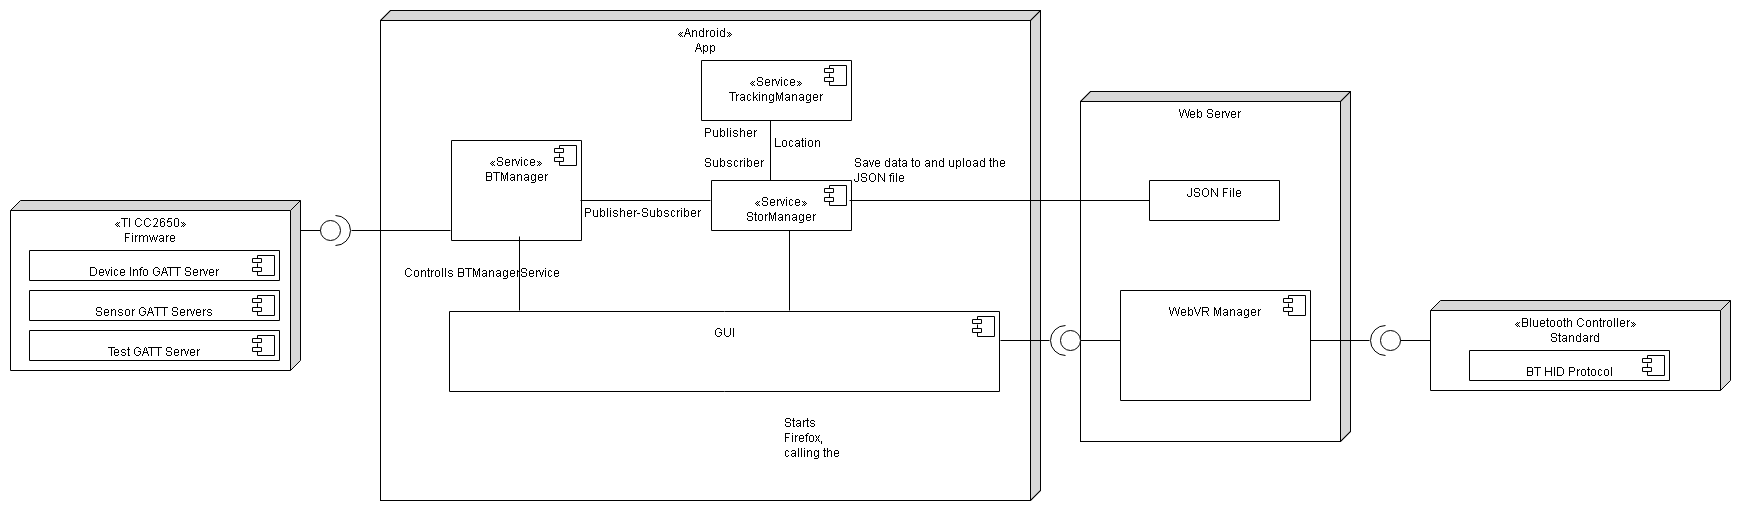
\includegraphics[width=1.4\textwidth]{pics/composite_app.png}


\subsection{Component Decomposition}

\subsubsection{Services}

\begin{itemize}
  \item \textbf{BluetoothManager:} Uses the android.bluetooth and especially the android.bluetooth.le libraries to fetch the sensor data from the sensor device. \\

 \hspace{-4cm} 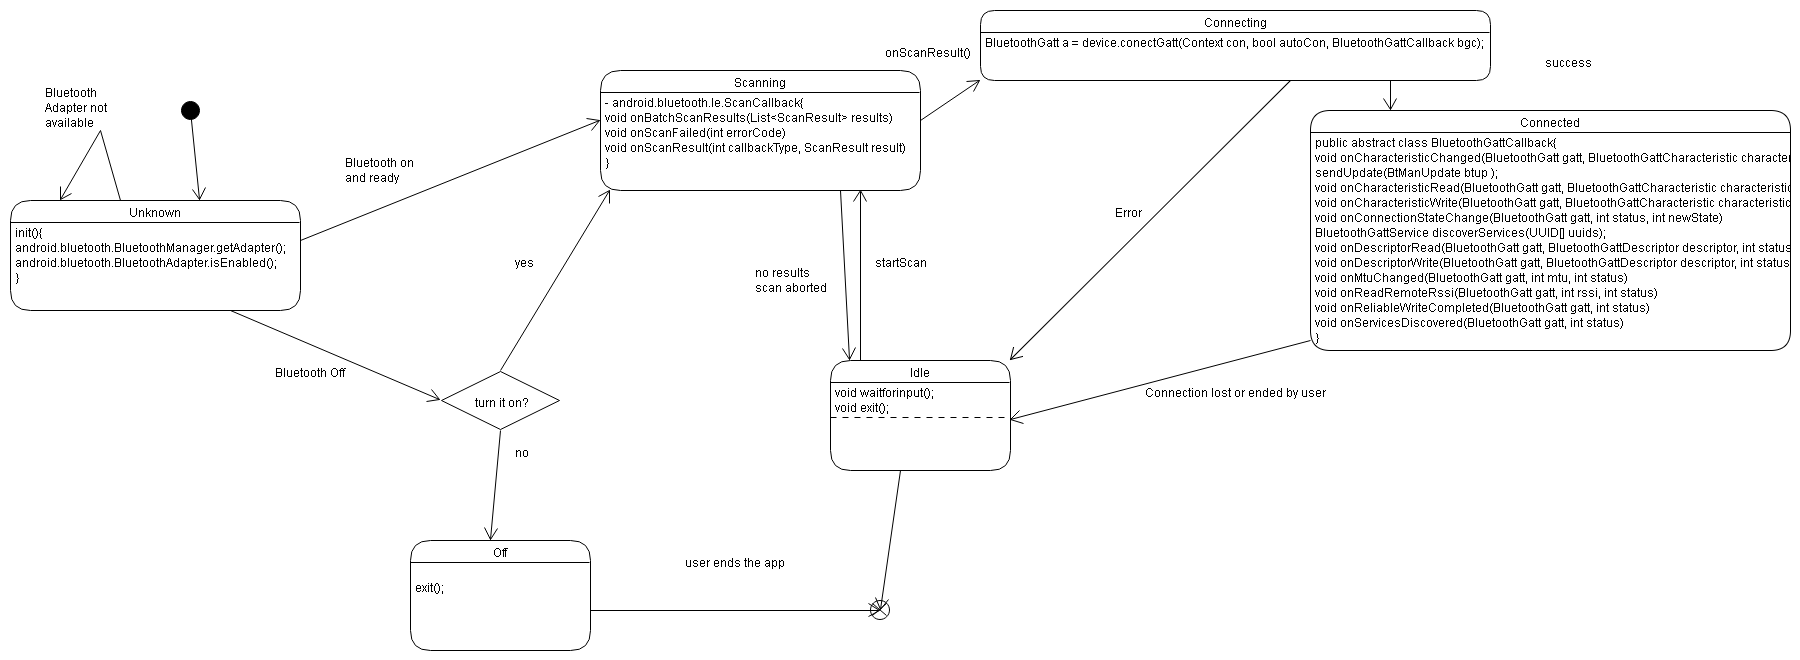
\includegraphics[width=1.4\textwidth]{pics/bt_state.png}

  \item \textbf{TrackingManager:} Handles the tracking of the (current) location where the data are recorded. The current position is determined by GPS and enhanced by the cellphone sensor and wifi data.

 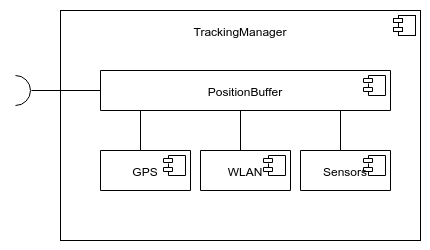
\includegraphics[width=0.8\textwidth]{pics/TrackingManager_Composition.png}

  \item \textbf{StorageManager:} Processes the data provided by the TrackingManager and the BluetoothManager. Uses a JSON file to store data.

 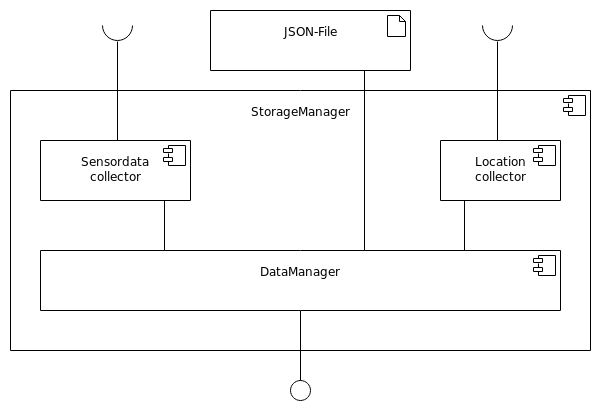
\includegraphics[width=0.8\textwidth]{pics/StorageMgr_Composition.png}

  \item \textbf{WebVRManager:} Handles the display of the virtual reality scene and the given data from the sensor.

 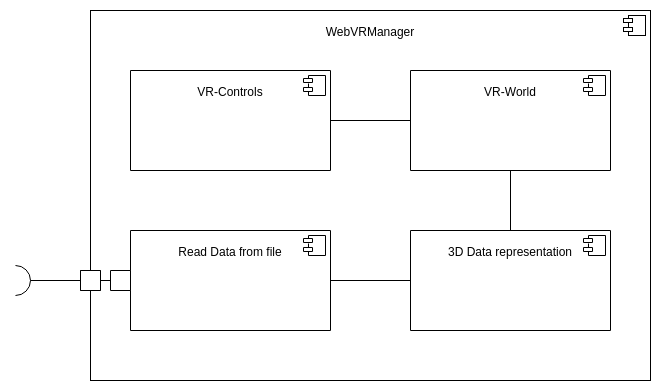
\includegraphics[width=0.8\textwidth]{pics/WebVRManager.png}

\end{itemize}

\subsubsection{GUI}

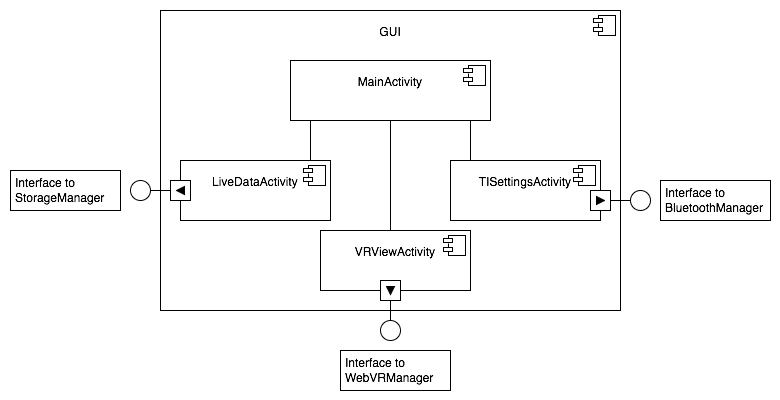
\includegraphics[width=0.8\textwidth]{pics/GUI.png}

\begin{itemize}
  \item \textbf{MainActivity} Provides the main startup screen as the main entry point.
  \item \textbf{VRViewActivity} Shall open a new browser window to display the WebVR webpage.
  \item \textbf{LiveDataActivity} Shall provide a view of the sensor data in human readable form.
  \item \textbf{TISettingsActivity:} Shall provide a settings screen containing scanning and connecting, connected devices and device settings fragments.
  \begin{itemize}
    \item \textbf{ScanningConnectingFragment} shall show the scanning results, delivered by the SensorTagBluetoothReceiverService and provide a connect on/off control.
    \item \textbf{ConnectedDevicesFragment} shall show the connected devices and a short info about the current setting and state of the sensor device.
    \item \textbf{ConnectedDevicesSettingsFragment} shall implement the configuration of the app features of the sensor.
  \end{itemize}
\end{itemize}

\subsubsection{Additional Classes}
\begin{itemize}
  \item \textbf{GATT Profiles} (for each sensor one)
  \item \textbf{GATT Sensor Service UUIDs}
  \item \textbf{Parser Functions} because the BLE protocol implemented in the TI CC2650 delivers raw sensor output
\end{itemize}

\subsection{Hardware/ Software mapping}

TO DO ???
\subsection{Persistent data management}
TO DO

\subsection{Global software control}
\subsubsection{Startup behavior}
\textbf{User:} The user can start the App by pressing the icon on his screen.
The App will show a startup screen and then transition after a short time into the main menu, from where
the user can start the other functions of the App.
\subsubsection{Interfaces}
The \textbf{BluetoothManager} provides a possibility to connect to a sensor and then read out
the data. It ensures that a connection is established and that the data is broad casted via a local BroadcastManager.
\\
\begin{lstlisting}
TODO pls add interfaces!
\end{lstlisting}

The \textbf{StorageManager} provides a possibility to store the data from the sensor together with th current position.
It also can store the data in a .json file an upload the data to a webserver.
\\
\begin{lstlisting}
InterfaceStorageManager {
  public void setSensor(integer internalSensorID){
    activeSensor = internalSensorID;
  }
  //tells the storage manager to get data from the active sensor and
  //the tracing manager, mark them with a timestamp and store the data
  //in a DataSet.
  public void measureNow(){
  }
  //get the latest measured DataSet of the active sensor
  public DataSet getLiveData() {
    return DataSet;
  }
  //get a DataSet which contains data of the activeSensor and position
  //at the specified time. If no data was stored at that time, an empty
  //DataSet will be returned.
  public DataSet getDataFrom(int time) {
    return DataSet;
  }
  //get multiple DataSets which contain all measured Data from the
  //active Sensor between 'time' and now.
  public DataSet[] getDataSince(int time) {
    return DataSet[];
  }
  // Upload the data set to a webserver
  // a .json file from time till now.
  public void uploadData(int time) {
    //upload the data to a server so webvr can later use it.
  }
}
\end{lstlisting}
The \textbf{TrackingManager} gets the current location of the smartphone and provides it to the rest of
the App.
\\
\begin{lstlisting}
Interface TrackingManager {
  //get the current location of the device
  public Location p getCurrentPosition() {
    ensures iff lockCustomPos
      p == customPos;
      else
        p == currentPosition;
  }
}
\end{lstlisting}

The \textbf{VRBox} gets the data from a webserver and loads it into the VR-World.
\\
\begin{lstlisting}
Interface WebVR {
  //Load the data from the webserver to display in VR.
  //The data will be a .json file which will be parsed
  // by in javascript by the web page.
  function loadData(file){
  }
}
\end{lstlisting}

\subsubsection{Sequences}

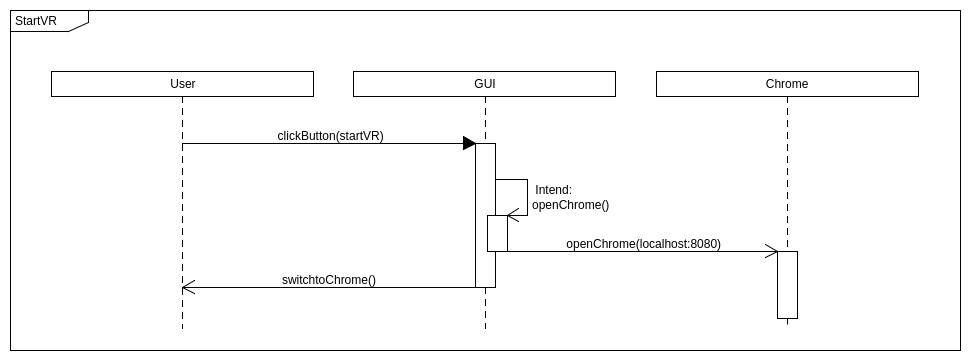
\includegraphics[width=0.8\textwidth]{diagramms/startVR.png}

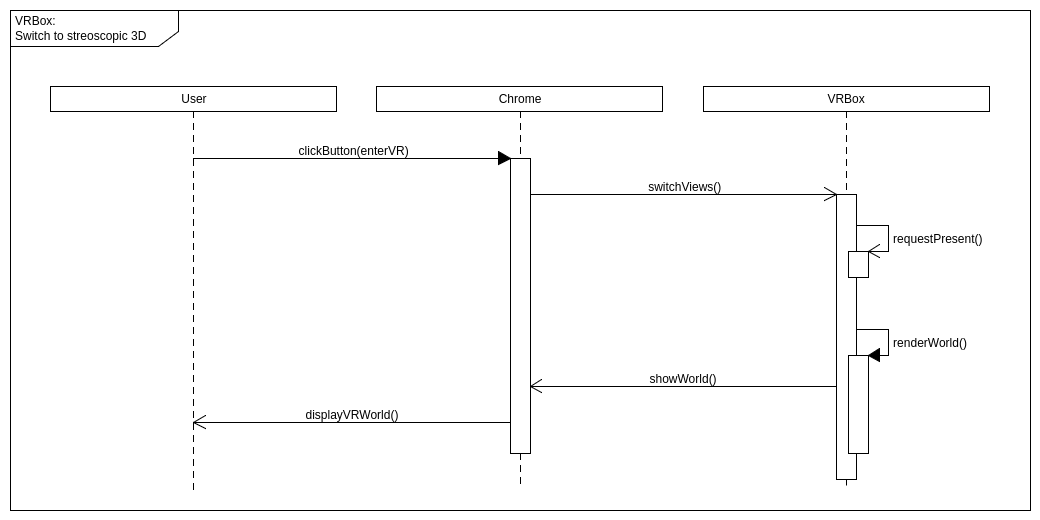
\includegraphics[width=0.8\textwidth]{diagramms/stereo.png}

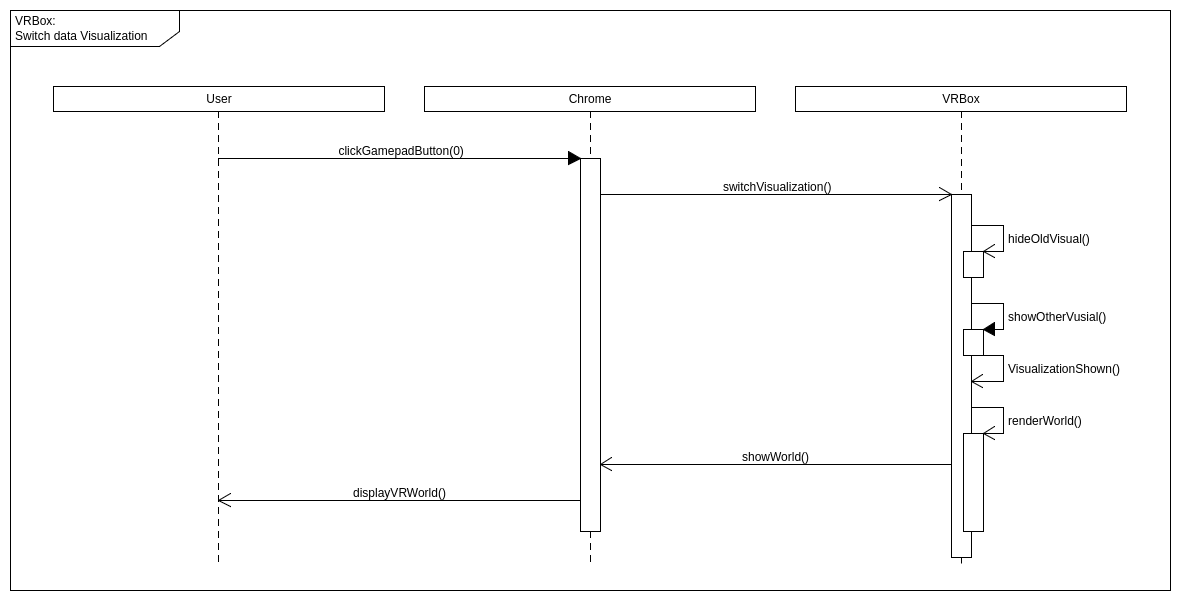
\includegraphics[width=0.8\textwidth]{diagramms/switchVisual.png}

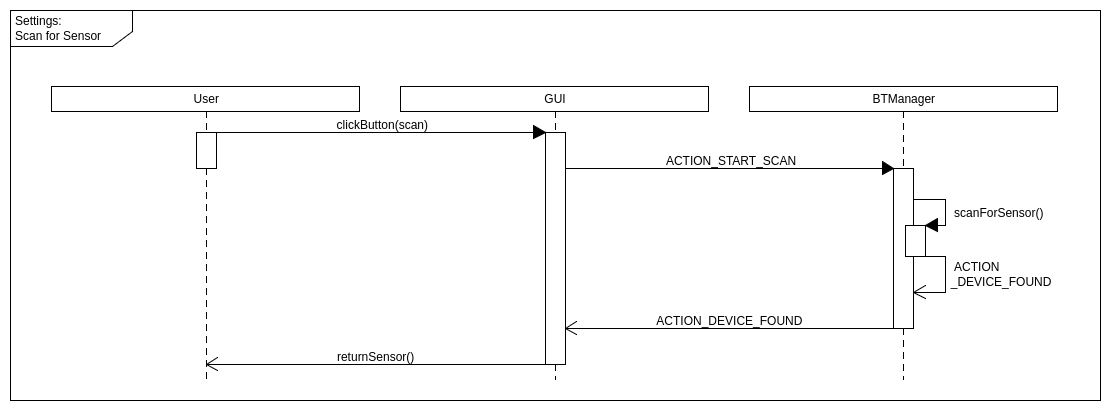
\includegraphics[width=0.8\textwidth]{diagramms/settingsScanForSensor.png}

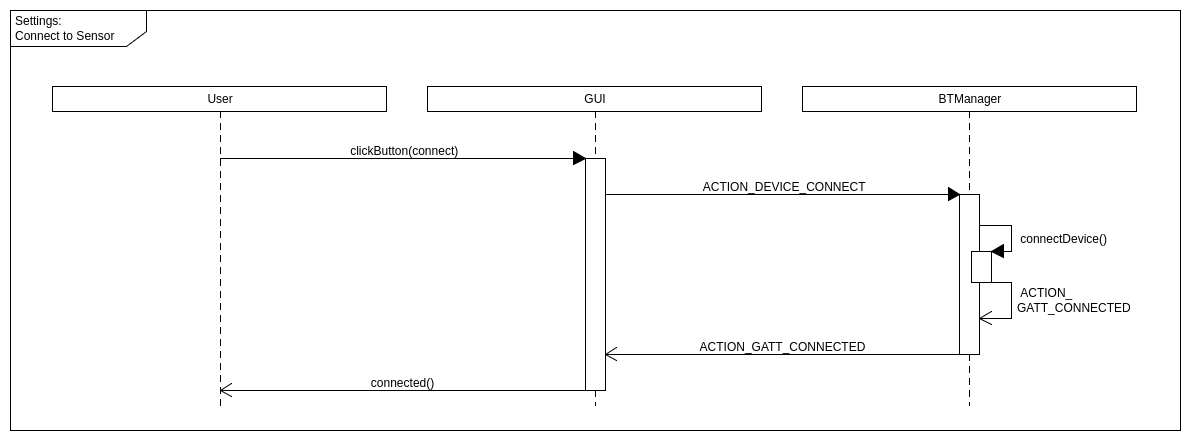
\includegraphics[width=0.8\textwidth]{diagramms/connectSensor.png}

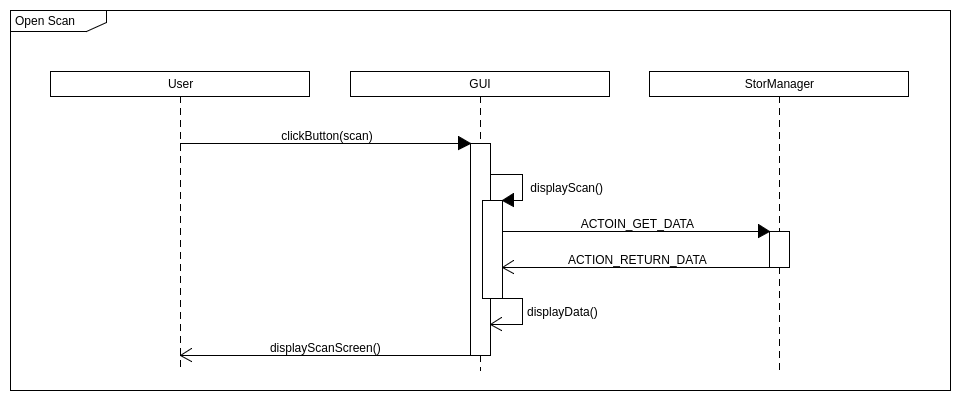
\includegraphics[width=0.8\textwidth]{diagramms/scan.png}

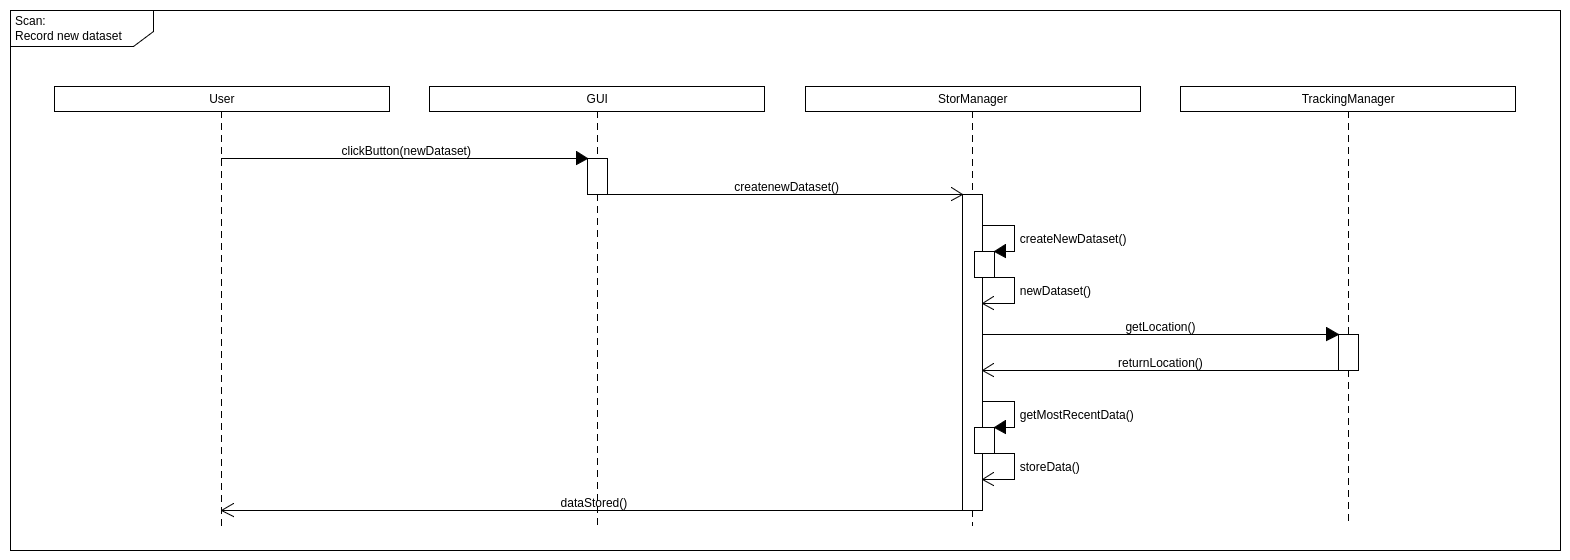
\includegraphics[width=0.8\textwidth]{diagramms/newDataset.png}

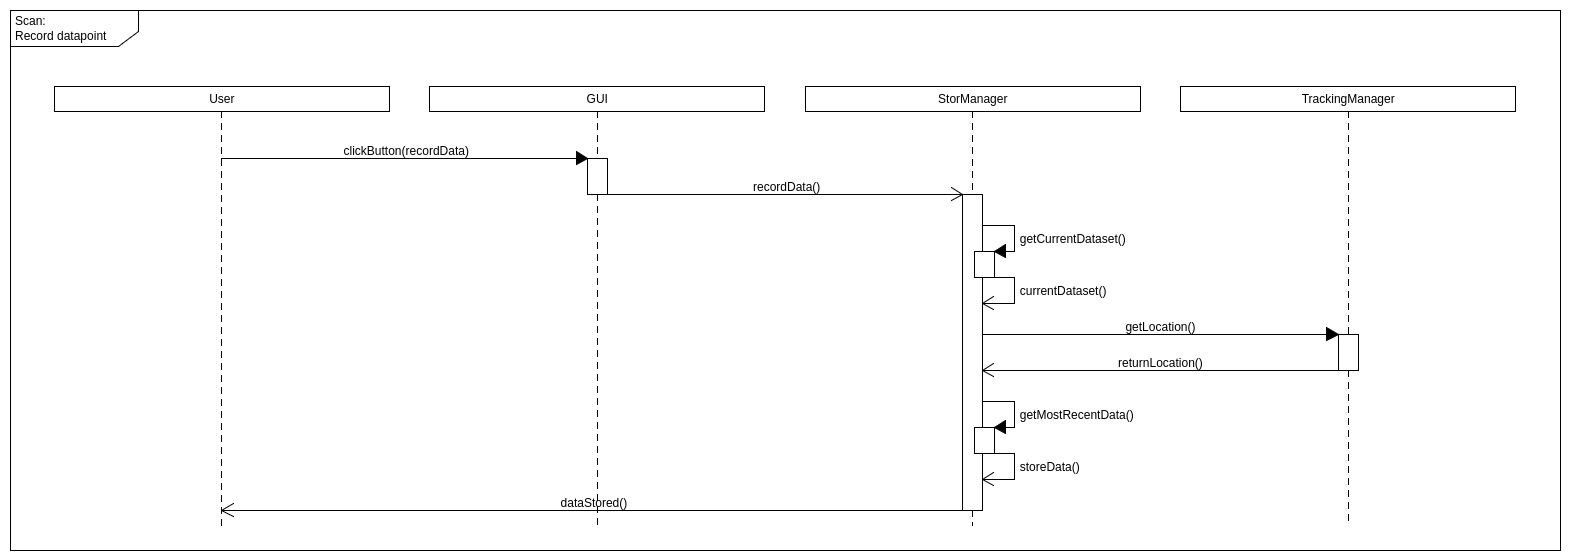
\includegraphics[width=0.8\textwidth]{diagramms/recordDatapoint.png}
